% Native LaTeX manuscript, authored from implementation and saved experiment data.
% Compile with Tectonic, or run pdfLaTeX twice. No conversion pipeline is used.
\documentclass[10pt,a4paper]{article}
\usepackage[T1]{fontenc}
\usepackage[utf8]{inputenc}
\usepackage[margin=23mm]{geometry}
\usepackage{amsmath,amssymb,graphicx,booktabs,array}
\usepackage{microtype,fancyhdr,float}
\usepackage[colorlinks=true,linkcolor=blue,citecolor=blue,urlcolor=blue]{hyperref}
\hypersetup{pdftitle={Weakly Supervised Temporal Localisation of Musical Instruments},pdfauthor={Ryan Hu}}
\setlength{\parskip}{4pt}
\setlength{\parindent}{0pt}
\setlength{\emergencystretch}{2em}
\pagestyle{fancy}\fancyhf{}
\fancyfoot[L]{\small ELEC5305 Project -- Ryan Hu (550275044)}
\fancyfoot[R]{\thepage}\renewcommand{\headrulewidth}{0pt}
\newcommand{\code}[1]{\texttt{\detokenize{#1}}}
\newcommand{\SelectedModel}{max}
\newcommand{\SelectedValidationBA}{0.787}
\newcommand{\ControlledFone}{0.587}
\newcommand{\ControlledBA}{0.609}
\newcommand{\ControlledSpecificity}{0.635}
\newcommand{\ControlledNegativeFone}{0.563}

\newcommand{\OriginalAttentionBA}{0.584}
\newcommand{\ControlledAttentionFoneBA}{0.620}
\newcommand{\ControlledAttentionBABA}{0.629}
\newcommand{\TrackDelta}{0.039}
\newcommand{\TrackLooLow}{0.034}
\newcommand{\TrackLooHigh}{0.044}
\newcommand{\BassFprDrumsOn}{0.503}
\newcommand{\BassFprDrumsOff}{0.276}

\setcounter{tocdepth}{1}
\begin{document}
\hypersetup{pageanchor=false}
\begin{titlepage}
\centering
\vspace*{12mm}
{\LARGE\bfseries Weakly Supervised Temporal Localisation of Musical Instruments\par}
\vspace{6mm}
{\large A controlled pooling comparison on BabySlakh and a 160-track Slakh2100-redux subset\par}
\vspace{14mm}
{\large Ryan Hu\par SID: 550275044\par}
\vspace{7mm}
ELEC5305 Acoustics, Speech and Signal Processing\\
The University of Sydney -- Semester 2, 2026
\vspace{10mm}

\href{https://github.com/Decarre/elec5305-project-550275044}{GitHub repository and working code}\\[3mm]
\href{https://decarre.github.io/elec5305-project-550275044/}{Project website}\\[3mm]
\href{https://github.com/Decarre/elec5305-project-550275044/blob/main/output/video/ELEC5305_Slakh160_Presentation_Polished.mp4}{Project demonstration video}
\vspace{10mm}
\begin{abstract}
Can a musical-instrument classifier trained with clip labels recover temporal activity? An initial BabySlakh experiment produced frame micro-F1 near 0.910, below an always-positive baseline at 0.915. A controlled follow-up added stem-remixed absence and transition scenes and compared mean, max and attention pooling across three seeds. A subsequent experiment sampled 160 tracks from the official Slakh2100-redux partitions (120 training, 20 validation and 20 test) and ran each pooling method with one seed. Training used clip labels, with MIDI activity used for temporal calibration and evaluation. In the 160-track experiment, max achieved the highest clip-validation macro balanced accuracy (0.814). Attention achieved the highest test frame macro balanced accuracy on original mixtures (0.707) and across all three variants (0.699), with pooled clip-local event F1 of 0.260. The enlarged experiment uses synthetic audio and a different test set from BabySlakh, leaving real-recording performance and the isolated effect of training-set size open.
\end{abstract}
\vfill
{\small Keywords: audio signal processing; weak supervision; instrument recognition; temporal localisation; attention pooling}
\end{titlepage}
\hypersetup{pageanchor=true}
\tableofcontents

\section{Introduction}
An instrument recogniser answers which instruments occur in an audio excerpt. A temporal localisation system must also determine when each instrument is active. This distinction matters for music navigation, arrangement analysis and visual activity timelines. In a polyphonic mixture, harmonic overlap, masking and instrument co-occurrence can make both decisions difficult. Clip labels are relatively inexpensive to obtain, whereas time-aligned reference activity requires additional annotation or isolated source information.

This project investigates the question: \emph{when training uses only clip-level instrument labels, do frame class scores and class-specific attention weights recover useful temporal activity?} The experiment changes the temporal aggregation rule while retaining the same encoder architecture, feature representation, data partitions and training settings. A global-mean model provides the learned comparison; an always-positive rule provides a necessary prevalence baseline.

The contribution is an implementation and evaluation study rather than a new state-of-the-art architecture. It separates frame scores, attention weights and clip predictions; protects the split against identical composition MIDI files; and evaluates clip recognition and temporal behaviour independently. An additional analysis of the saved confusion counts exposes the difficulty of interpreting F1 when nearly every clip contains most target families.

Three questions make that contribution testable: (1) does the clip-validation winner also provide the best temporal discrimination; (2) does the controlled training-data condition improve temporal performance when checkpoint selection is held fixed; and (3) are false positives associated with the activity of another instrument? The pooling comparison, factorial ablation and conditional-error analysis address these questions respectively.

\section{Background and related work}
\subsection{Weak labels and instrument recognition}
Gururani, Sharma and Lerch formulate instrument recognition from weak labels using an attention mechanism and report improved recognition on OpenMIC \cite{attentionmic}. Their study motivates learning class-specific contributions over time. The present implementation adopts bounded frame scores and normalised attention aggregation, but uses a compact convolutional encoder and a different dataset. It is therefore a study of the aggregation idea, not an exact reproduction of the published experimental system.

A clip marked positive need contain only one active interval for an instrument. Consequently, minimising clip classification loss does not uniquely determine a frame activity function. A classifier may respond to a short cue, or to another source correlated with the target. Evaluating clip accuracy alone cannot resolve this ambiguity. This report explicitly assesses frame scores and compares attention mass with a uniform reference.

Kong et al. describe class-specific attention as a learned distribution over instances in a weakly labelled audio bag \cite{kongattention}. This supplies a useful distinction between the instance score and the measure used to aggregate it. Wang et al. compare multiple-instance pooling functions with explicit attention to localisation \cite{milpooling}. Their results caution that a pooling rule successful for tagging need not be the best for localisation. The present study tests this distinction with matched encoders rather than assuming the clip-validation winner will produce the best timeline.

OpenMIC contains partially labelled real-music excerpts \cite{openmic}, making it relevant to recognition but insufficient by itself for a temporally referenced comparison. MedleyDB supplies multitrack recordings and instrument activations \cite{medleydb}. The latter motivated the original dataset choice, but full local audio was unavailable for the completed experiment. This limitation is retained rather than describing BabySlakh as an equivalent real-recording benchmark.

\subsection{Synthetic mixtures and temporal references}
Slakh provides synthesized musical mixtures and corresponding stems generated from MIDI \cite{slakh}. MIDI timing makes it possible to derive temporal references without manually annotating every mixture. The study starts with BabySlakh \cite{babyslakhrelease} and extends the pooling comparison to a 160-track subset of Slakh2100-redux \cite{slakhredux}. Synthesized mixtures offer controlled access to timing information, but their timbres, arrangements and production conditions cannot represent the full diversity of recorded music.

MIDI note activity is also a particular target definition. It captures note intervals, not necessarily audible energy: a source can decay after note-off, reverberation can persist, and an active note can be masked by louder sources. A score against MIDI activity should be described with that reference definition rather than presented as perfect perceptual localisation.

Gururani, Summers and Lerch study instrument activity detection using MedleyDB and Mixing Secrets \cite{iad}. They derive labels from stem energy and train at time scales down to one second. Their supervised activity targets differ from the five-second presence labels used for model training here.

\subsection{Attention as a diagnostic}
Jain and Wallace examine limitations of treating attention as explanation in natural-language models \cite{jain}. Those experiments do not directly establish a result for audio. They motivate the narrower methodological choice here: measure alignment rather than assume it. A time-normalised attention weight expresses a relative contribution within one clip and class. It does not have the same interpretation as the probability that an instrument is active at a particular time.

\subsection{Position relative to pretrained representations}
PANNs demonstrates transfer of AudioSet-pretrained networks to audio tasks \cite{panns}; MERT develops self-supervised music representations using acoustic and musical teachers \cite{mert}. These methods motivate future transfer experiments and could address the limited diversity of a small training collection. They do not remove the need for temporal references, leakage controls or an appropriate operating point. This project's compact encoder was retained to study pooling and signal semantics at modest computational cost, not to claim state-of-the-art instrument recognition.

\section{Data and experimental protocol}
\subsection{Completed scope}
Full MedleyDB access remained pending when the fallback experiment was prepared. The initial experiments use BabySlakh at 16\,kHz with drums, bass, guitar and piano as target families. The BabySlakh split has 12 training, four validation and four test tracks, yielding 562, 190 and 212 complete five-second clips respectively. The 160-track follow-up retains the same target families and is detailed in Section~\ref{sec:slakh160}. Partial trailing clips are discarded.

\begin{table}[htbp]
\centering
\caption{BabySlakh split sizes. Clips are created after assigning track groups.}
\label{tab:split}
\begin{tabular}{lrr}\toprule
Partition & Tracks & Five-second clips\\\midrule
Training & 12 & 562\\
Validation & 4 & 190\\
Test & 4 & 212\\\bottomrule
\end{tabular}
\end{table}

\subsection{Grouping before clipping}
The adapter computes SHA-256 hashes of each track's \code{all_src.mid}. It shuffles the sorted set of hash groups with seed 5305, then assigns groups to approximately 60\% training, 20\% validation and 20\% test. All tracks sharing one hash stay together. An explicit assertion checks that a hash never crosses partitions before audio is divided into clips.

This barrier detects byte-identical MIDI files. It does not establish that all musically equivalent arrangements, related compositions or alternative MIDI serialisations are independent. Likewise, multiple clips from the same test track remain correlated. The 212 test clips must not be interpreted as 212 independent musical works.

\subsection{Reference construction and weak supervision}
Stem metadata maps each supported instrument to one of the four families. Notes from the mapped stem MIDI files are combined within each family. For bin $b$ and class $c$, the binary reference is
\begin{equation}
r_{bc}=\mathbf{1}\{\text{at least one class-$c$ note overlaps bin $b$}\}.
\end{equation}
Each five-second clip has ten nominal 0.5\,s reference bins. The clip label is $y_c=\max_b r_{bc}$. The training interface receives features and these four clip labels; it does not use the bin references as a training target. Separate temporal archives are available for validation and test analysis. Thus temporal labels inform threshold selection during validation, even though optimisation of the neural networks uses only clip labels.

\section{Signal processing and models}
\subsection{Log-mel representation}
Mixtures are loaded as mono audio at 16\,kHz. A 1024-sample FFT and a 320-sample hop produce a short-time power representation. The power spectrum is projected onto 64 mel bands. The preparation script uses a per-clip maximum as the dB reference and scales the clipped values:
\begin{equation}
X_{mt}=\frac{1}{80}\operatorname{clip}\left(10\log_{10}\frac{P_{mt}}{P_{\max}},-80,0\right).
\end{equation}
Numerical floors are handled by the library implementation. Features therefore lie approximately in $[-1,0]$. Per-clip normalisation removes absolute recording-level information; it does not separate overlapping instruments.

\subsection{Common frame encoder}
All pooling variants use two temporal convolutions with 64 hidden channels, kernel sizes five and three, and padding that retains the time axis. Each convolution is followed by batch normalisation and ReLU. There is no temporal downsampling. With frame feature $h_t$, a linear class head produces
\begin{equation}
p_{tc}=\sigma(w_c^\top h_t+b_c).
\end{equation}
These bounded scores are candidate frame activity estimates. Their training objective constrains the aggregated clip output, so their probabilistic calibration at frame level is not guaranteed.

\subsection{Pooling alternatives}
The mean model aggregates frame probabilities directly:
\begin{equation}
\widehat y^{\mathrm{mean}}_c=\frac{1}{T}\sum_{t=1}^{T}p_{tc}.
\end{equation}
The attention model adds one linear head, followed by a sigmoid and normalisation across time:
\begin{align}
u_{tc}&=\sigma(v_c^\top h_t+d_c), &
a_{tc}&=\frac{u_{tc}}{\sum_{s=1}^{T}u_{sc}},\\
\widehat y^{\mathrm{att}}_c&=\sum_{t=1}^{T}a_{tc}p_{tc}, &
\sum_t a_{tc}&=1.
\end{align}
The implementation clamps the denominator for numerical stability. Both alternatives use the same architecture for encoding and class scoring, but they are trained separately; they do not share fitted weights. Attention also introduces extra parameters, so this comparison isolates an aggregation design rather than enforcing identical parameter counts.

Max pooling uses $\widehat y_c^{\max}=\max_t p_{tc}$. Holding attention weights fixed, the pooling derivatives with respect to frame scores are $1/T$ for mean, $a_{tc}$ for attention, and one at an argmax (zero elsewhere, away from ties) for max. Mean spreads the clip-loss signal; max concentrates it on a few cues. This offers a mechanism for tagging and activity coverage to diverge, consistent with \cite{milpooling}. Seed instability alone does not establish sparse gradients as its cause.

\subsection{Optimisation and selection}
The models minimise clip-level binary cross-entropy using Adam with learning rate $10^{-3}$ and batch size 32. Training is capped at 30 epochs with patience six. At each epoch, class thresholds are selected on validation predictions from the grid $\{0.05,0.10,\ldots,0.95\}$. In the initial experiment, the checkpoint with the best validation macro-F1 is retained; training loss breaks checkpoint ties. Threshold ties prefer values nearer 0.5, then the smaller value. The controlled follow-up changes the selection objective to balanced accuracy; Table~\ref{tab:protocols} distinguishes the protocols.

Seeds 5305, 5306 and 5307 vary training randomness on the same dataset split. Their standard deviation describes variation across these training runs, not uncertainty over different track samples. Clip test evaluation reuses thresholds stored with the selected checkpoint. Frame thresholds are fitted separately on the validation temporal references and kept fixed for the main test comparison.

\section{Evaluation}
\subsection{Clip and temporal metrics}
For each class, $F_1=2TP/(2TP+FP+FN)$. Micro-F1 pools counts over classes and samples; macro-F1 averages the four class F1 values. For temporal evaluation the runner divides the model's frame axis into ten nearly equal groups and averages scores in each group. It sums attention weights within each group, preserving total attention mass. Because feature frames are grouped by array index, these are nominal 0.5\,s bins rather than a sample-exact STFT-to-MIDI timestamp alignment.

The initial runner reports bin-level F1 and does not produce event-matching or onset/offset-error results. The follow-up in Section~\ref{sec:controlled} adds timestamp binning and a separate event evaluator. Smoothing and minimum-event-duration fields in the initial configuration are not applied by its bin-scoring path.

\subsection{Attention alignment}
For a positive clip and class, let $A_c=\sum_b a_{bc}r_{bc}$ be attention mass on active bins and $q_c=B^{-1}\sum_b r_{bc}$ be the active-bin fraction. The lift is
\begin{equation}\ell_c=A_c/q_c.
\end{equation}
Uniform attention gives lift one. Lift is calculated per positive clip and then averaged. A large active mass alone is weak evidence when $q_c$ is already close to one. Classes absent from a clip are excluded from this diagnostic.

\subsection{Prevalence baseline and sensitivity}
An always-positive predictor requires no learned parameters or threshold fitting. If a class is positive in $n_c$ of $N$ samples, its F1 is $2n_c/(N+n_c)$. This baseline is derived from the saved test confusion counts; it was added during the report audit without changing model checkpoints. It is a diagnostic comparison, not a new training run.

The existing sensitivity analysis adds $-0.10$, zero or $+0.10$ to each selected frame threshold and clips the result to $[0.01,0.99]$. These are post-hoc test diagnostics. None replaces the validation-selected operating point in the main table.

\section{Initial experiment and diagnostic audit}
\begin{table}[H]\centering\small
\caption{Test performance: mean and sample standard deviation over three training seeds on one fixed split. The deterministic baseline has no seed variability.}\label{tab:main}
\begin{tabular}{lrrrr}\toprule
Model & \shortstack{Clip\\micro-F1} & \shortstack{Clip\\macro-F1} & \shortstack{Frame\\micro-F1} & \shortstack{Frame\\macro-F1} \\\midrule
Mean & $0.946 \pm 0.012$ & $0.942 \pm 0.015$ & $0.910 \pm 0.004$ & $0.902 \pm 0.006$ \\
Attention & $0.950 \pm 0.008$ & $0.948 \pm 0.009$ & $0.910 \pm 0.011$ & $0.901 \pm 0.018$ \\
Always positive & 0.962 & 0.961 & 0.915 & 0.910 \\
\bottomrule\end{tabular}\end{table}

\subsection{Recognition and temporal discrimination}
Table~\ref{tab:main} shows a clip micro-F1 advantage of approximately 0.004 for attention over mean pooling. The frame micro-F1 difference is below 0.0001 and favours mean pooling before rounding. This small set of three seeds does not establish a reliable improvement in temporal localisation. More decisively, neither learned model exceeds the always-positive rule on aggregate clip or frame micro-F1.

The positive-bin counts for drums, bass, guitar and piano are 2040, 2023, 1395 and 1697 out of 2120 bins per class. Overall, 7155 of 8480 class-bin labels are positive. In this setting, F1 rewards high recall and does not count true negatives. A predictor that marks nearly everything active can therefore receive a superficially strong score. The results demonstrate execution of a weak-label pipeline but not useful localisation beyond a prevalence-only strategy.

The supplementary material retains the initial Track00012 example. Several class scores decline together when piano stops, illustrating why a plot alone does not establish class-specific boundary discrimination.

\subsection{Class behaviour and attention}
\begin{table}[H]\centering\small
\caption{Frame F1 by class, averaged across seeds. Positive counts are recovered from TP+FN and agree across models and seeds.}\label{tab:classes}
\begin{tabular}{lrrrr}\toprule
Class & Positive bins & Mean & Attention & Always positive \\\midrule
drums & 2040/2120 & 0.979 & 0.983 & 0.981 \\
bass & 2023/2120 & 0.976 & 0.981 & 0.977 \\
guitar & 1395/2120 & 0.765 & 0.751 & 0.794 \\
piano & 1697/2120 & 0.889 & 0.889 & 0.889 \\
\bottomrule\end{tabular}\end{table}

Table~\ref{tab:classes} exposes variation hidden by micro averages. Guitar is harder than drums and bass, and the attention model's guitar frame F1 varies substantially by seed. Piano frame F1 is identical across the saved runs. Inspection of its confusion rows shows 1697 true positives, 423 false positives and no false negatives: the thresholded predictions mark every piano bin active. Its apparent temporal F1 therefore comes entirely from prevalence.

Mean attention lift over the twelve class-by-seed rows is 1.013. Positive clips have active fractions of approximately 0.976 for drums, 0.968 for bass, 0.762 for guitar and 0.917 for piano. Attention mass on active bins is consequently high even for nearly uniform weights. The lift supplies little evidence of strong concentration beyond that uniform reference.

\subsection{Threshold and co-occurrence effects}
\begin{table}[H]\centering\small
\caption{Post-hoc threshold sensitivity, averaged across seeds. Main results use the zero-offset row.}\label{tab:sensitivity}
\begin{tabular}{lrrr}\toprule
Model & Offset & Frame micro-F1 & Frame macro-F1 \\\midrule
mean & -0.10 & 0.914 & 0.908 \\
mean & +0.00 & 0.910 & 0.902 \\
mean & +0.10 & 0.887 & 0.874 \\
attention & -0.10 & 0.918 & 0.912 \\
attention & +0.00 & 0.910 & 0.901 \\
attention & +0.10 & 0.843 & 0.808 \\
\bottomrule\end{tabular}\end{table}

Table~\ref{tab:sensitivity} shows that decreasing thresholds raises micro-F1, whereas increasing them lowers it, particularly for attention. This is consistent with dense positive labels making recall especially valuable; it does not prove that lower thresholds would improve practical boundary detection. Test-set selection of a better offset would compromise the evaluation protocol and has not been performed.

Drums and bass co-occur in 206 of the 212 clips with at least one of them present, giving Jaccard overlap 0.972. Such association makes it difficult to distinguish recognition of an instrument from reliance on common arrangements. Controlled negative examples and isolated changes in source activity would provide a stronger test.

\section{Controlled follow-up and optimisation}
\label{sec:controlled}
The initial experiment identified a measurement problem: dense positive labels allowed high F1 without useful rejection of inactive intervals. The follow-up therefore changes the data coverage and evaluation protocol before comparing temporal behaviour. Table~\ref{tab:protocols} summarises the changes; the later factorial analysis separates two of these factors.

\begin{table}[H]
\centering\small
\caption{Protocol differences. All stages preserve the same track partition and use clip labels for neural-network training. BA denotes macro balanced accuracy.}
\label{tab:protocols}
\begin{tabular}{p{.23\linewidth}p{.31\linewidth}p{.34\linewidth}}\toprule
Component & Initial experiment & Controlled follow-up\\\midrule
Training scenes & Original mixtures & Original, absence and transition scenes\\
Pooling candidates & Mean, attention & Mean, attention, max\\
Clip selection objective & Validation macro-F1 & Validation macro BA\\
Frame evaluation & Index bins; validation-F1 thresholds & Timestamp bins; validation-BA thresholds\\
Temporal outcomes & Bin F1 and attention lift & Balanced and negative-class measures; clip-local events\\\bottomrule
\end{tabular}
\end{table}

\subsection{Protocol fixed before retraining}
The initial diagnostic motivated a separate controlled benchmark. The source tracks and their split remain fixed. Each source clip yields three scenes: its original mixture; a mixture with two randomly selected target families completely removed; and a mixture where every target family switches on or off once at a randomly selected 0.5 s boundary between 1.5 and 3.5 s. Other instrument stems remain as background. The intervention generator seeds each scene from SHA-256 of the track, clip index, scene type and protocol version. It does not inspect labels or model success when choosing gates.

For remixed scenes, available stems are summed by instrument family, multiplied by the corresponding time gate, and mixed with the remaining stems. A five-millisecond ramp around each switch reduces discontinuities. Original scenes retain the supplied mixture. Temporal references are the intersection of the original MIDI references and the applied gates. This construction uses isolated sources to create data and labels; the models still receive mixture features and clip labels only. It is not a source-free augmentation method.

The resulting partitions contain 1686 training, 570 validation and 636 test scenes. Every derivative inherits its source track's partition; there are still only four independent test tracks. Original scenes and artificial scenes are reported separately. Masking improves negative-class coverage but does not create new compositions or independent musical performances.

\subsection{Evaluation and model changes}
The revised evaluator assigns centred STFT frames by timestamps $t\times320/16000$ to half-open reference bins. The frame centred exactly at five seconds is excluded. Frame scores are averaged within physical bins; attention mass, when aggregated, is renormalised over retained frames. A boundary fixture verifies both the first and final bins.

Specificity is $TN/(TN+FP)$, negative-class F1 is $2TN/(2TN+FP+FN)$, and balanced accuracy is the mean of sensitivity and specificity. Undefined rates are retained as missing, rather than assigned a perfect score. Always-positive, always-negative and training-prevalence constant predictors are saved as baselines. A constant rule has balanced accuracy 0.5 when both classes occur.

All three pooling models use the existing encoder and hyperparameters. Max pooling is added as a candidate because local discriminative cues need not occupy most of a clip. Checkpoints and clip thresholds now maximise validation macro balanced accuracy, and frame thresholds are selected on validation temporal labels using the same objective. The candidate model is selected by mean validation clip macro balanced accuracy over seeds, before examining its test advantage. This selects \SelectedModel{} (validation score \SelectedValidationBA{}). These are fixed candidate comparisons, not a broad hyperparameter search.

Legacy checkpoints are also re-evaluated with timestamp bins and newly calibrated validation-balanced frame thresholds. Their original training and checkpoint-selection rule remain unchanged. Consequently, the transfer table compares complete training protocols; it cannot attribute every change specifically to augmentation or checkpoint selection.

\begin{table}[H]\centering\small
\caption{Controlled test frame precision, recall and F1, with imbalance-aware complements. Means across three seeds; operating points are fixed by controlled validation. See the supplement and saved results for variability and negative-class F1.}\label{tab:controlled}
\begin{tabular}{lrrrrrr}\toprule
Model & Micro P & Micro R & Micro F1 & Macro F1 & Macro BA & Specificity \\\midrule
baseline & 0.615 & 0.700 & 0.655 & 0.647 & 0.589 & 0.472 \\
attention & 0.658 & 0.754 & 0.702 & 0.689 & 0.629 & 0.515 \\
max & 0.654 & 0.580 & 0.587 & 0.576 & 0.609 & 0.635 \\
always positive & 0.562 & 1.000 & 0.720 & 0.716 & 0.500 & 0.000 \\
always negative & 0.000 & 0.000 & 0.000 & 0.000 & 0.500 & 1.000 \\
training prevalence & 0.562 & 1.000 & 0.720 & 0.716 & 0.500 & 0.000 \\
\bottomrule\end{tabular}\end{table}
\begin{table}[H]\centering\small
\caption{Identical timestamp-based frame evaluator with validation-balanced threshold calibration for all checkpoints. Legacy models retain their original training and checkpoint selection.}\label{tab:transfer}
\begin{tabular}{lrr}\toprule
Training/model & Original subset BA & Controlled BA \\\midrule
legacy attention & 0.627 & 0.570 \\
legacy mean & 0.590 & 0.559 \\
retrained attention & 0.659 & 0.629 \\
retrained baseline & 0.596 & 0.589 \\
retrained max & 0.621 & 0.609 \\
\bottomrule\end{tabular}\end{table}
\subsection{Temporal stress tests}
The validation-selected model achieves controlled-test micro-F1 \ControlledFone{}, macro balanced accuracy \ControlledBA{}, specificity \ControlledSpecificity{} and negative-class F1 \ControlledNegativeFone{}. Table~\ref{tab:variants} separates natural-subset scenes from controlled absence and transition scenes. Performance on the original subset remains a separate check for distribution change.

Attention has the highest descriptive controlled-test macro balanced accuracy, 0.629 versus 0.589 for mean and 0.609 for max pooling. The legacy attention checkpoints reach 0.570 under the same new evaluator, while retrained attention reaches 0.629. This is a combined protocol improvement, not an isolated causal estimate of the augmentation effect. The predeclared clip-validation rule selects max pooling, whose test micro-F1 has a large seed standard deviation (0.189). This mismatch between clip selection and temporal performance is a limitation; a future experiment should predeclare temporal validation selection rather than retrospectively switching the winner using this test set.

\begin{table}[H]\centering\small
\caption{Validation-selected model on separately reported scene types. Event F1 is clip-local with a 0.5 s endpoint tolerance.}\label{tab:variants}
\begin{tabular}{lrrrrr}\toprule
Scene & Micro-F1 & Macro BA & Specificity & Neg.-F1 & Event F1 \\\midrule
original & 0.667 & 0.621 & 0.649 & 0.291 & 0.271 \\
absence & 0.525 & 0.604 & 0.633 & 0.624 & 0.166 \\
transition & 0.524 & 0.608 & 0.646 & 0.639 & 0.220 \\
\bottomrule\end{tabular}\end{table}
Clip-local events are contiguous runs of positive bins. One-to-one matching requires both endpoints to fall within 0.5 s of the reference event. Matching maximises the number of valid pairs before minimising endpoint error. Events touching clip boundaries are censored there; these scores do not measure continuous-track onset and offset detection. Matched onset/offset mean absolute errors and unmatched-event counts are saved for each run and scene type. A low matched error alone can hide many unmatched events, so event F1 is reported alongside it.

\begin{figure}[H]\centering
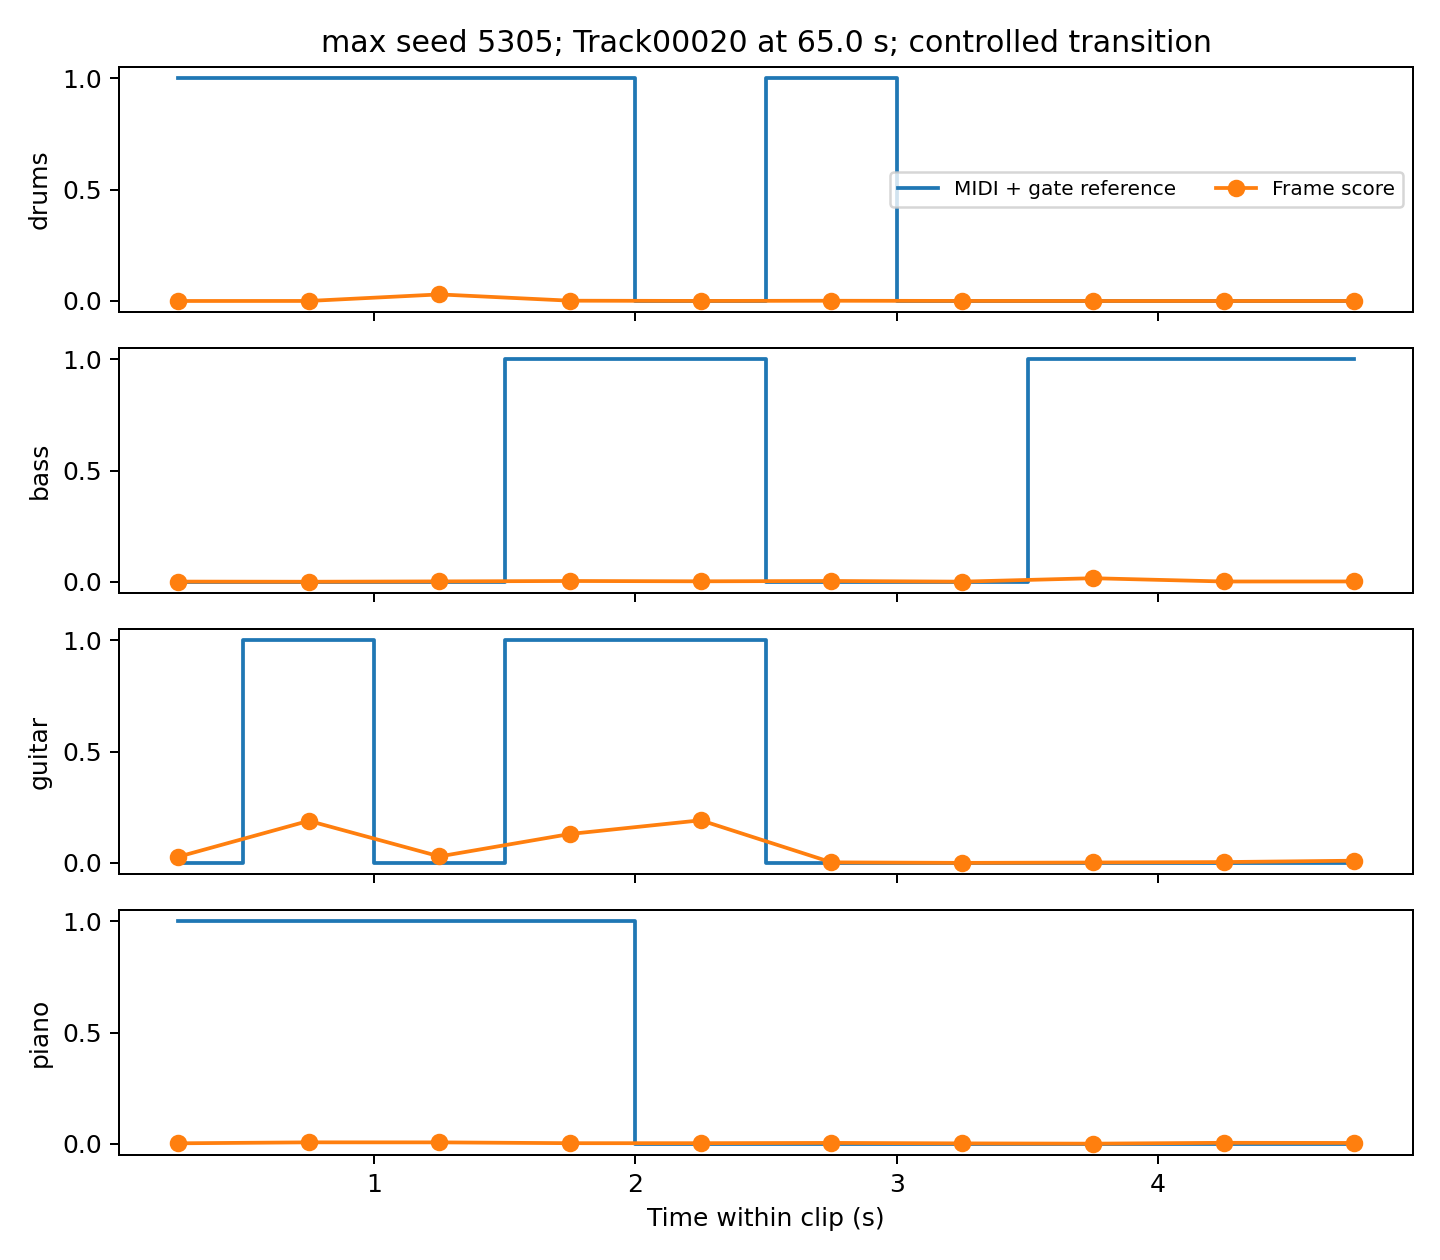
\includegraphics[width=.78\linewidth]{figures/controlled_transition.png}
\caption{Controlled transition example for the validation-selected architecture, seed 5305. Selection maximises reference transitions, with the first clip breaking ties; it does not select successful predictions. Each panel separates the binary gated MIDI reference from the frame score. Artificial switching and MIDI activity are not perceptual ground truth for natural recordings.}
\label{fig:controlled}
\end{figure}

\section{Signal diagnostics and explanatory analyses}
The controlled comparison establishes the main model results. The following analyses examine what the output signals represent, which protocol changes accompany the improvement, and where false positives occur. They use the same inspected test tracks and retain the original model choice and operating point.
\subsection{Frame scores, attention and weighted contribution}
Frozen-checkpoint diagnostics compare frame scores, attention and the relative weighted contribution on controlled data. The contribution $a_{tc}p_{tc}$ is time-normalised only for relative alignment, not interpreted as activity probability. Each signal has separate validation-F1 calibration. Across attention seeds, diagnostic micro-F1 is 0.733 for frame scores, 0.720 for attention and 0.715 for contribution. These operating points differ from the validation-balanced calibration in the main controlled comparison, so the values answer a separate signal-comparison question.

Attention lift averages 1.055 on original scenes and 1.519 on artificial transition scenes; contribution lift on transitions is 1.597. Thus artificial switching produces relative alignment but does not establish calibrated activity. The full per-class/scene alignment and primary frame precision/recall/F1 tables accompany the report in the supplementary PDF and result CSV files.

Validation-only threshold offsets ($\pm0.10$) and smoothing windows (one, three or five 0.5 s bins) are also recorded. At the original thresholds, attention validation macro balanced accuracy changes from 0.714 without smoothing to 0.719/0.717 with three/five bins. The frozen test operating point is retained. Sensitivity is assessed without choosing a new setting from test performance; all 81 measurements are supplied.

\subsection{Training-data and selection factors}
A retrospective $2\times2$ ablation crosses original/controlled training scenes with F1/balanced-accuracy clip selection for mean and attention pooling. Twelve new and twelve retained runs cover eight conditions with three seeds each, keeping frame evaluation fixed. Under balanced selection, attention's controlled-test frame BA is \OriginalAttentionBA{} with original training data and \ControlledAttentionBABA{} with controlled training. Controlled training under F1 selection reaches \ControlledAttentionFoneBA{}. The supplement gives paired-seed contrasts. This separates two protocol factors, but the data factor still includes extra scenes and training exposure, and these test tracks were already inspected.

\subsection{Track stability and conditional errors}
Retrained attention exceeds mean on each of the four test tracks. The unweighted controlled-track BA difference averages \TrackDelta{}; leaving out any one track gives \TrackLooLow{}--\TrackLooHigh{}. This checks sensitivity to the sampled tracks without treating clips or seeds as independent musical works; it is not a population confidence interval.

With bass absent, bass FPR averaged over the three attention seeds is \BassFprDrumsOn{} when drums are active (1235 reference bins) and \BassFprDrumsOff{} when drums are absent (1055 bins). Thus co-occurrence is associated with a measurable error difference, beyond the overlap of clip labels alone. The supplement supplies conditional contrasts and denominators; causal interpretation is considered in the discussion.


\section{Expanded experiment on 160 Slakh2100-redux tracks}
\label{sec:slakh160}

\subsection{Data and training}
The follow-up samples tracks with seed 5305 from the official Slakh2100-redux training, validation and test partitions \cite{slakhredux}. The pinned download manifest identifies all tracks and source files. An assertion checks that identical full-track MIDI hashes do not cross partitions. Mono audio is resampled to 16\,kHz and split into complete five-second clips. Each clip has an original mix, a two-family absence mix and a mix with controlled starts or stops. The 120 training, 20 validation and 20 test tracks yield 17,670, 2,985 and 3,051 examples including all variants. The test partition contains 1,017 original clips.

Mean, max and attention pooling use the same encoder and clip-label loss. Each model was trained once with seed 5305. Checkpoints were selected by validation clip macro balanced accuracy. Frame thresholds were calibrated on the validation MIDI references and fixed for test evaluation. Event scoring uses a 0.5\,s tolerance at both endpoints with clip-edge censoring, as in the BabySlakh follow-up.

\subsection{Recognition and localisation results}
\begin{table}[htbp]
\centering
\small
\caption{Results on the 160-track subset, one run per pooling method. Frame BA is macro balanced accuracy. Pooled results combine the original, absence and transition variants.}
\label{tab:slakh160}
\begin{tabular}{lrrrrr}
\toprule
Pooling & Val.\ clip BA & Test clip BA & Original frame BA & Pooled frame BA & Pooled event F1\\
\midrule
Mean & 0.740 & 0.740 & 0.689 & 0.682 & 0.228\\
Max & \textbf{0.814} & \textbf{0.819} & 0.635 & 0.652 & 0.108\\
Attention & 0.790 & 0.784 & \textbf{0.707} & \textbf{0.699} & \textbf{0.260}\\
\bottomrule
\end{tabular}
\end{table}

Max pooling led clip-level validation and test recognition. Attention scored highest on frame-level test localisation for original mixes and for the pooled variants (Table~\ref{tab:slakh160}). On absence and transition mixes, its frame BA was 0.703 for each after rounding. The pooled always-active baseline achieved frame BA of 0.500. Attention's pooled event F1 of 0.260 shows that locating complete intervals remains difficult, even when many individual bins are classified correctly.

\clearpage
\subsection{Validation examples shown in the demonstration}
\begin{figure}[H]
\centering
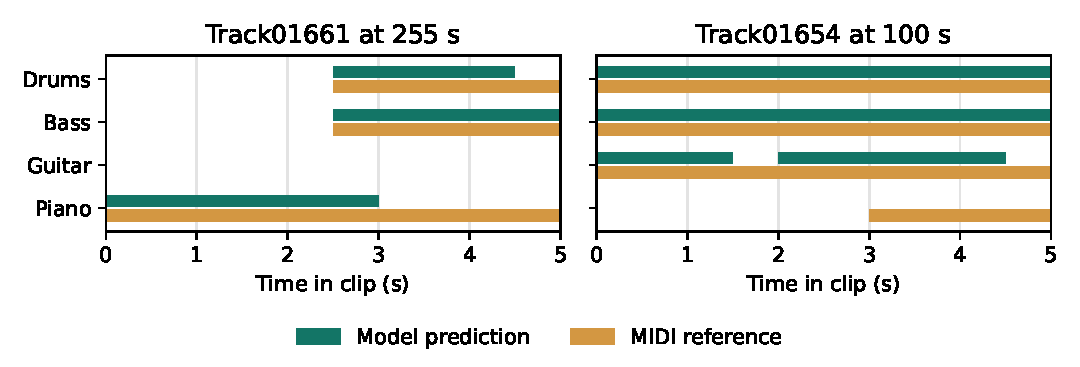
\includegraphics[width=\linewidth]{figures/slakh160_demo.pdf}
\caption{Attention checkpoint outputs and MIDI reference activity for two selected validation excerpts. Times are relative to each five-second clip. The excerpts illustrate a matching bass onset and a missed piano interval.}
\label{fig:slakh160-demo}
\end{figure}

In \code{Track01661}, the predicted and reference bass intervals begin at 2.5\,s and extend to the clip boundary. In \code{Track01654}, the MIDI reference shows piano activity from 3.0 to 5.0\,s and the model produces no piano interval (Figure~\ref{fig:slakh160-demo}). The video shows inference on the WAV excerpts. These examples are selected from the validation set and the aggregate scores come from the held-out test partition.

The BabySlakh and 160-track experiments use different held-out tracks. Comparing 0.629 with 0.699 describes results on those two evaluations. A shared test set and matched training protocol would be needed to estimate the effect of increasing the training set. The single-seed follow-up also leaves between-run variation unmeasured.


\section{Discussion}
\subsection{Answers to the research questions}
\textbf{Clip selection and temporal discrimination.} In both the controlled BabySlakh comparison and the 160-track experiment, max pooling ranks highest under the clip-validation rule and attention ranks highest on test frame balanced accuracy across the three scene variants. The initial experiment also shows why a high frame F1 is insufficient when positive bins dominate. These findings support choosing a validation objective that matches the intended application. The reported test rankings are descriptive.

\textbf{Controlled training with fixed checkpoint selection.} The factorial comparison supports a positive association within this benchmark: under balanced selection, attention improves from \OriginalAttentionBA{} to \ControlledAttentionBABA{}, with an improvement also present under F1 selection. Controlled scenes therefore contribute beyond the choice of checkpoint objective. However, they add training examples and exposure as well as different activity patterns; the experiment does not isolate the acoustic intervention alone. The positive attention-versus-mean difference on every test track makes a single-track explanation less likely.

\textbf{Contextual activity and false positives.} Bass false positives are more frequent when drums are active, even after restricting the analysis to bins where bass is absent. This connects the co-occurrence concern to actual errors, but it cannot identify the model's causal mechanism. Arrangement, masking and the intervention procedure remain competing explanations.

These answers also clarify the role of attention. Its relative alignment improves on artificial transitions, but normalised attention mass remains distinct from an activity probability. Weak clip supervision can reward a useful cue without requiring complete active-interval coverage. This explains why the report evaluates frame scores and attention separately; it does not contradict the recognition results of \cite{attentionmic}, which concern a different dataset and task.

\subsection{Threats to validity}
\textbf{Limited sampling.} BabySlakh has four held-out synthetic tracks and the enlarged experiment has twenty. Clips within each track remain correlated. BabySlakh has three training seeds on a fixed split and the enlarged experiment has one run per pooling method. Neither design estimates uncertainty across independent music collections.

\textbf{Reference and alignment.} MIDI note overlap differs from audible activity, and 0.5\,s bins obscure short gaps and attacks. The follow-up replaces index grouping with physical timestamps, but quantisation and the STFT analysis window still limit timing precision. Event scoring uses the stated tolerance and clip-edge censoring.

\begin{samepage}
\textbf{Label prevalence and intervention design.} Selecting four common families creates few negative clips and long positive regions in the original mixtures, where the always-positive baseline outperforms both initial models on aggregate F1. The controlled scenes improve negative coverage but may introduce switching cues absent from natural music, despite the short ramps. Their temporal discrimination therefore needs an independent transfer test.
\par\end{samepage}

\textbf{Model selection.} Validation is used for both checkpoint and threshold selection on a small set of tracks. This is preferable to test tuning, but it can still overfit the validation partition. The sensitivity analysis reveals dependence on operating point. A larger validation set or nested development protocol would give a more stable comparison.

\textbf{Scope of grouping.} Hash grouping protects against byte-identical files only. It should be supplemented by composition metadata or canonicalised note representations before broader claims about composition independence.

\subsection{Next experiments}
The next scale comparison should train on nested subsets and evaluate on the same held-out tracks with a fixed validation protocol. This would separate training-set size from the change in test repertoire. External evaluation on real recordings would address generalisation beyond synthetic audio. Comparing MIDI references with stem-energy activity would test reference sensitivity, while a supervised frame model would help quantify the cost of weak training labels.

\section{Conclusion}
Weakly supervised instrument recognition can produce high frame F1 without useful temporal discrimination, as the initial prevalence baseline demonstrates. In the 160-track follow-up, max led clip-level validation and attention led frame-level test results, with macro balanced accuracy of 0.707 on original mixes and 0.699 across all variants. Its pooled clip-local event F1 of 0.260 shows that complete intervals remain difficult to recover. The BabySlakh factorial and conditional-error analyses provide additional evidence on training condition and instrument co-occurrence. The results support evaluating clip recognition, activity timing and attention alignment separately. The effect of scaling on a common test set and generalisation to real recordings remain open.

\section*{Reproducibility and acknowledgements}
The website and video links appear on the title page. The script \code{download_slakh_subset.py} fetches the 160-track sample. The script \code{run_slakh2100.py} prepares the data and evaluates the models. The demonstration uses the trained attention checkpoint and its validation-derived calibration. The \code{predict} command accepts audio and exports scores, activity intervals and a timeline using the training feature transform. The supplementary PDF and \code{REPRODUCE.md} document the BabySlakh experiments.

Generative AI assisted code development, report drafting, source inspection and LaTeX typesetting. Initial measurements come from retained experiment outputs; the follow-up and factorial measurements come from the documented training runs. The initial always-positive result is calculated from saved confusion counts. Responsibility for the submitted analysis, implementation and source attribution rests with the author.

\clearpage
% Publication metadata checked against primary publication records.
\begin{thebibliography}{10}
\bibitem{attentionmic} S. Gururani, M. Sharma, and A. Lerch,
``An Attention Mechanism for Musical Instrument Recognition,''
in \emph{Proceedings of ISMIR}, 2019, pp. 83--90.
\url{https://arxiv.org/abs/1907.04294}.
\bibitem{slakh} E. Manilow, G. Wichern, P. Seetharaman, and J. Le Roux,
``Cutting Music Source Separation Some Slakh: A Dataset to Study the Impact of Training Data Quality and Quantity,''
in \emph{IEEE WASPAA}, 2019, pp. 45--49.
\url{https://doi.org/10.1109/WASPAA.2019.8937170}.
\bibitem{jain} S. Jain and B. C. Wallace,
``Attention is not Explanation,'' in \emph{Proceedings of NAACL-HLT},
2019, pp. 3543--3556.
\url{https://doi.org/10.18653/v1/N19-1357}.
\bibitem{medleydb} R. M. Bittner, J. Salamon, M. Tierney, M. Mauch,
C. Cannam, and J. P. Bello, ``MedleyDB: A Multitrack Dataset for
Annotation-Intensive MIR Research,'' in \emph{ISMIR}, 2014, pp. 155--160.
\url{https://zenodo.org/records/1417889}.
\bibitem{openmic} E. J. Humphrey, S. Durand, and B. McFee,
``OpenMIC-2018: An Open Dataset for Multiple Instrument Recognition,''
in \emph{ISMIR}, 2018.
\url{https://brianmcfee.net/papers/ismir2018_openmic.pdf}.
\bibitem{kongattention} Q. Kong, Y. Xu, W. Wang, and M. D. Plumbley,
``Audio Set Classification with Attention Model: A Probabilistic Perspective,''
in \emph{ICASSP}, 2018, pp. 316--320.
\url{https://doi.org/10.1109/ICASSP.2018.8461392}.
\bibitem{milpooling} Y. Wang, J. Li, and F. Metze,
``A Comparison of Five Multiple Instance Learning Pooling Functions for Sound
Event Detection with Weak Labeling,'' in \emph{ICASSP}, 2019.
\url{https://arxiv.org/abs/1810.09050}.
\bibitem{iad} S. Gururani, C. Summers, and A. Lerch,
``Instrument Activity Detection in Polyphonic Music using Deep Neural Networks,''
in \emph{ISMIR}, 2018, pp. 569--576.
\url{https://archives.ismir.net/ismir2018/paper/000275.pdf}.
\bibitem{panns} Q. Kong, Y. Cao, T. Iqbal, Y. Wang, W. Wang, and M. D. Plumbley,
``PANNs: Large-Scale Pretrained Audio Neural Networks for Audio Pattern Recognition,''
\emph{IEEE/ACM TASLP}, vol. 28, pp. 2880--2894, 2020.
\url{https://doi.org/10.1109/TASLP.2020.3030497}.
\bibitem{mert} Y. Li et al., ``MERT: Acoustic Music Understanding Model with
Large-Scale Self-supervised Training,'' in \emph{ICLR}, 2024.
\url{https://arxiv.org/abs/2306.00107}.
\end{thebibliography}

\end{document}
